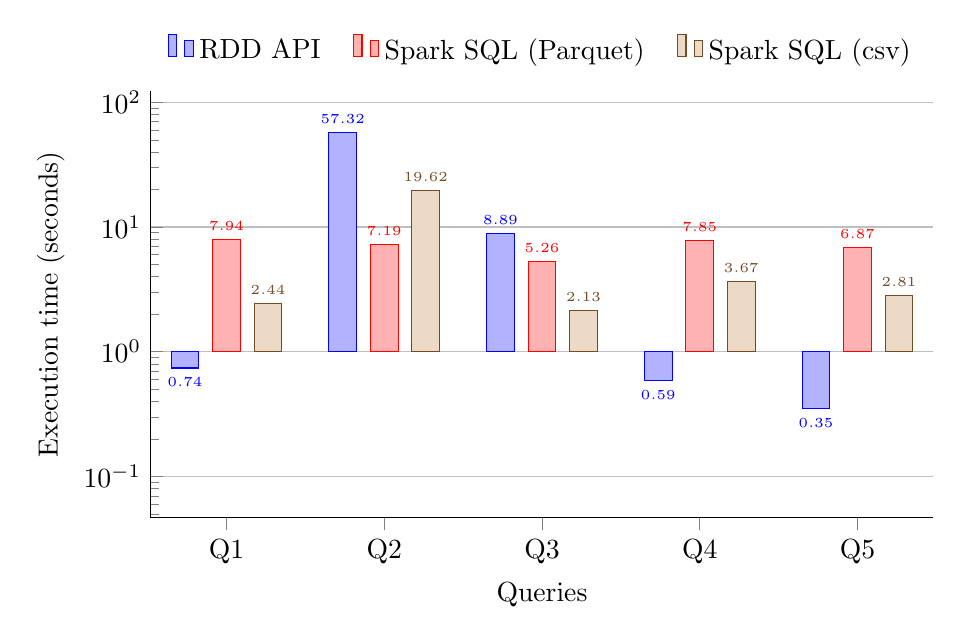
\begin{tikzpicture}
\begin{axis}[
    ybar=5pt,
    enlargelimits=0.12,
    bar width=10pt,
    ylabel={Execution time (seconds)},
    xlabel={Queries},
    width=0.95\textwidth,
    height=7cm,
    symbolic x coords={Q1,Q2,Q3,Q4,Q5},
    xtick=data,
    ymode=log,
    ymin=0.1,
    ymajorgrids=true,
    axis x line* = bottom,
    axis y line* = left,
    legend style={cells={anchor=west}, draw=none},
    legend style={at={(0.5,1.15)}, anchor=north,legend columns=-1},
    legend columns=-1,
    point meta=explicit symbolic,
    nodes near coords=\pgfmathprintnumber{\pgfplotspointmeta},
    visualization depends on={y<0.2?0:1 \as \myshift},
    every node near coord/.append style={font=\tiny, anchor=north, yshift=(\myshift*10pt)},
    ]
\addplot table [meta=Y] {
  X Y
  Q1  0.74
  Q2 57.32
  Q3  8.89
  Q4  0.59
  Q5  0.35
};

\addplot table [meta=Y] {
  X Y
  Q1  7.94
  Q2  7.19
  Q3  5.26
  Q4  7.85
  Q5  6.87
};

\addplot table [meta=Y] {
  X Y
  Q1  2.44
  Q2 19.62
  Q3  2.13
  Q4  3.67
  Q5  2.81
};

\legend{RDD API\hphantom{xz}, Spark SQL (Parquet)\hphantom{xz} , Spark SQL (csv) }
\end{axis}
\end{tikzpicture}